\documentclass[journal]{IEEEtran}

\usepackage{amsmath,amssymb,amsfonts}
\usepackage{algorithmic}
\usepackage{graphicx}
\usepackage{textcomp}
\usepackage{xcolor}
\usepackage{booktabs}
\usepackage{cite}
\usepackage{url}
\usepackage{microtype}

\begin{document}

\title{BotDriftBench: An Empirically Calibrated Synthetic Longitudinal Benchmark for Drift-Aware Social Bot Detection}

\author{Eshan~Amballa%
\thanks{E. Amballa is with the Department of Computer Science and Engineering. Email: eshanikaamballa@gmail.com.}}

\maketitle

\begin{abstract}
Evaluating social bot detectors under non-stationary deployment requires longitudinal benchmark data with verifiable drift ground truth---a resource absent from existing cross-sectional datasets. We introduce \textbf{BotDriftBench v0.8}, an empirically calibrated synthetic longitudinal benchmark specifically constructed for drift-aware social bot detection. The benchmark encompasses 3,000 unique accounts (1,500 human, 1,500 bot) tracked over 20 temporal windows, generating 60,000 observations across 25 profile and behavioral features. Marginal distributions are fitted from the verified subset of TwiBot-22 (294,478 humans, 38,986 bots) and cross-validated against Cresci-2017. Seven account-level drift scenarios inject longitudinal shifts into targeted feature groups, including boundary-crossing evasion (20\%), gradual evasion (26\%), abrupt evasion (10\%), localized evasion (8\%), recurring behavior (6\%), behavioral gradual evolution (17\%), and stationary controls (13\%). Version 0.8 introduces four major methodological advances: (1) core profile counters (\textit{account\_age\_days}, \textit{followers\_count}, \textit{friends\_count}, \textit{listed\_count}) evolve via monotonic organic growth dynamics rather than artificial coordinate interpolation; (2) human reference manifolds are constructed by sampling complete empirical training rows to preserve multi-dimensional covariance structures; (3) train/val/test partitioning strictly precedes human-manifold construction to eliminate reference leakage; and (4) an account-disjoint 3-way evaluation protocol (1,800 train / 600 validation / 600 test accounts) evaluated across 5 random seeds (2025--2029). Benchmark validation reveals that a frozen static detector suffers severe performance degradation under evasion drift (Macro-F1 falling from 0.9770 to 0.8059 post-drift; worst window F1 = 0.6583), while localized drift-aware adaptation recovers performance to 0.9167 F1. BotDriftBench v0.8 is publicly released under CC BY 4.0 with complete generative code for reproducible evaluation.
\end{abstract}

\begin{IEEEkeywords}
Benchmark dataset, social bot detection, concept drift, synthetic data generation, TwiBot-22, temporal evaluation, longitudinal benchmark, account-disjoint split.
\end{IEEEkeywords}

\section{Introduction}
\IEEEPARstart{S}{upervised} machine learning classifiers have achieved strong accuracy in identifying automated accounts on static social media corpora~\cite{cresci2017paradigm,feng2022twibot}. However, the standard cross-sectional evaluation paradigm assesses models at a single temporal snapshot, assuming that feature distributions observed during training persist unchanged throughout deployment. 

In production environments, bot architectures continually adapt to avoid platform suspensions and moderation filters~\cite{ferrara2016rise,hays2025bots}. This adversarial evolution produces concept drift and covariate shift~\cite{gama2014survey}, degrading static classifiers silently. 

Evaluating drift detection and adaptation algorithms requires longitudinal benchmarks with known drift ground truth: exact onset windows, targeted feature groups, and verified account labels. Existing public benchmarks fail to satisfy these requirements:
\begin{itemize}
    \item \textbf{Absence of Drift Ground Truth}: In real-world data streams, behavioral shifts confound genuine adversarial adaptation with platform API changes, breaking news cycles, and organic human habit evolution.
    \item \textbf{Data Access and Privacy Obstacles}: Platform API restrictions, paywalls, and privacy mandates severely impede the public distribution of longitudinal raw tweet corpora.
    \item \textbf{Unstandardized Evaluation Splits}: Variable partitioning schemes undermine reproducibility across independent investigations.
\end{itemize}

BotDriftBench v0.8 resolves these limitations by providing an empirically calibrated synthetic longitudinal benchmark where drift onset, affected features, and evasion mechanisms are rigorously controlled and fully documented.

\section{Related Benchmarks and Limitations}
Prominent social bot benchmarks, such as Cresci-2017~\cite{cresci2017paradigm} and TwiBot-22~\cite{feng2022twibot}, have driven significant algorithmic advances. However, they are cross-sectional: accounts are evaluated on static holdout splits without temporal progression. While longitudinal studies have documented behavioral changes in the wild~\cite{hays2025bots}, they lack controlled labels indicating when and how individual accounts drifted, precluding systematic evaluation of drift detectors.

\section{Benchmark Architecture and Cohort Design}

\begin{figure}[!t]
\centering
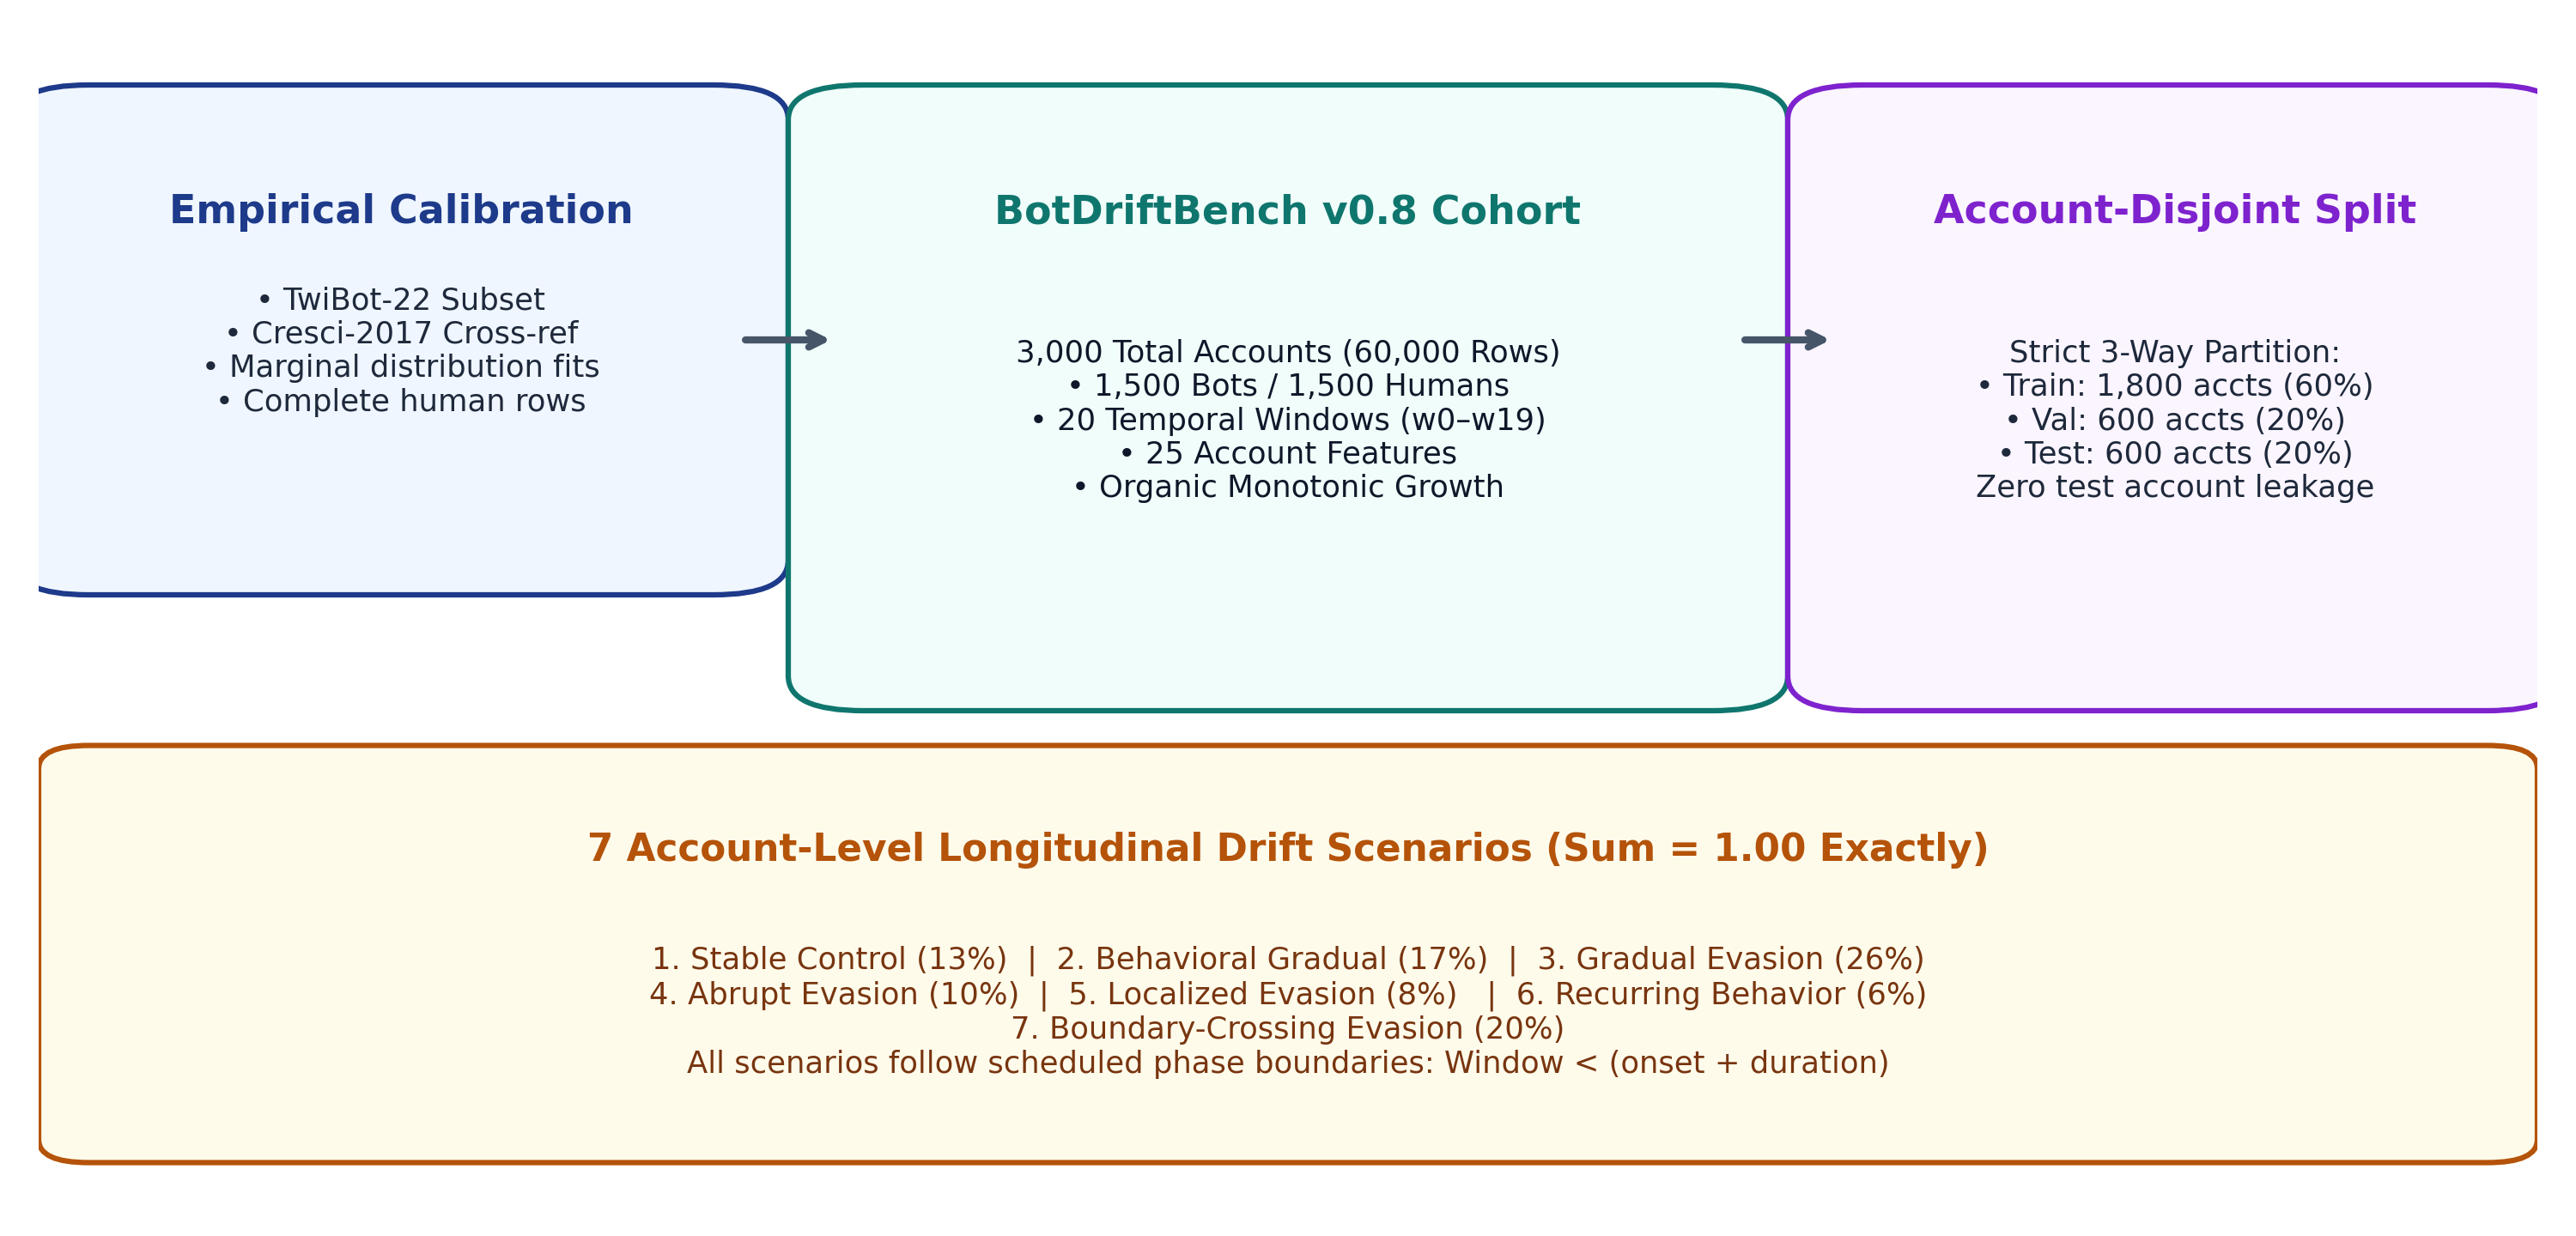
\includegraphics[width=\columnwidth]{paper_pictures/fig1_benchmark_architecture.png}
\caption{BotDriftBench v0.8 architectural workflow: empirical calibration from TwiBot-22 and Cresci-2017, organic growth modeling, strict 3-way account-disjoint partitioning, and 7 longitudinal drift scenarios.}
\label{fig:architecture}
\end{figure}

BotDriftBench v0.8 comprises 3,000 unique accounts tracked across 20 discrete temporal windows ($t \in [0, 19]$), yielding 60,000 observation vectors $\mathbf{x}_{i,t} \in \mathbb{R}^{25}$:
\begin{itemize}
    \item \textbf{Profile Features (10)}: \textit{account\_age\_days}, \textit{statuses\_count}, \textit{followers\_count}, \textit{friends\_count}, \textit{listed\_count}, \textit{description\_length}, \textit{screen\_name\_length}, \textit{verified\_score}, \textit{reputation\_score}, \textit{caps\_ratio}.
    \item \textbf{Behavioral Features (15)}: \textit{tweets\_per\_day}, \textit{posting\_regularity}, \textit{night\_post\_ratio}, \textit{weekend\_post\_ratio}, \textit{burst\_score}, \textit{text\_entropy}, \textit{vocabulary\_richness}, \textit{emoji\_ratio}, \textit{content\_similarity}, \textit{reply\_ratio}, \textit{retweet\_ratio}, \textit{mention\_ratio}, \textit{hashtag\_count\_avg}, \textit{url\_ratio}, \textit{conversation\_depth}.
\end{itemize}

\subsection{Organic Profile Growth Dynamics}
Earlier benchmark iterations interpolated profile counters toward target coordinates, introducing unphysical artifacts (e.g., account age reversing). BotDriftBench v0.8 enforces monotonic organic growth:
\begin{equation}
\text{age}_{i, t} = \text{age}_{i, 0} + 30 \cdot t,
\end{equation}
\begin{equation}
\text{followers}_{i, t} = \text{followers}_{i, 0} \cdot (1 + \gamma_{\text{growth}})^t, \quad \gamma_{\text{growth}} \sim \mathcal{N}(\mu_g, \sigma_g^2),
\end{equation}
reflecting realistic operational constraints: bot operators cannot instantaneously forge multi-year account histories or large organic followings.

\section{Empirical Calibration and Separability}

\begin{figure}[!t]
\centering
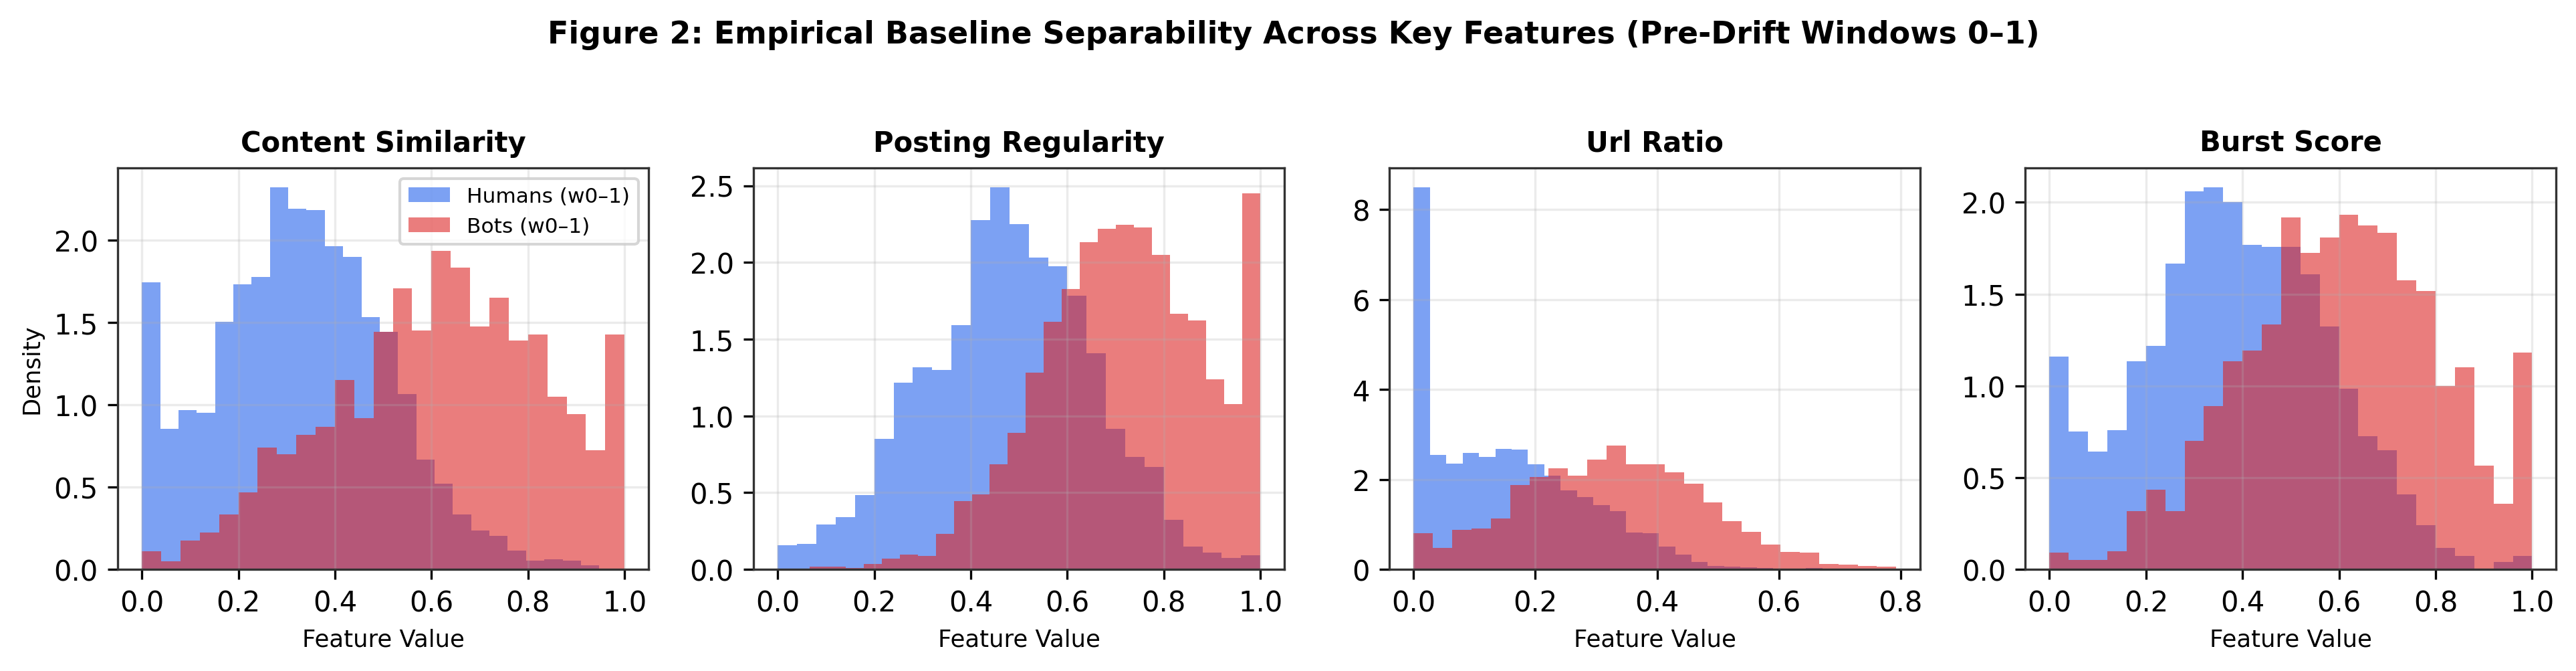
\includegraphics[width=\columnwidth]{paper_pictures/fig2_feature_separability.png}
\caption{Pre-drift feature separability (Windows 0--1) between human accounts (blue) and bot accounts (red) across key behavioral dimensions.}
\label{fig:separability}
\end{figure}

Marginal distributions were fitted from the verified subset of TwiBot-22~\cite{feng2022twibot} (294,478 humans, 38,986 bots) and cross-validated against Cresci-2017~\cite{cresci2017paradigm}. Bounded ratio features were modeled with Beta distributions, count metrics with log-normal distributions, and binary features with Bernoulli trials.

To prevent covariance distortion, synthetic human target vectors are sampled as complete training rows rather than independent feature draws, preserving empirical cross-feature correlations.

\section{Controlled Longitudinal Drift Scenarios}

\begin{figure}[!t]
\centering
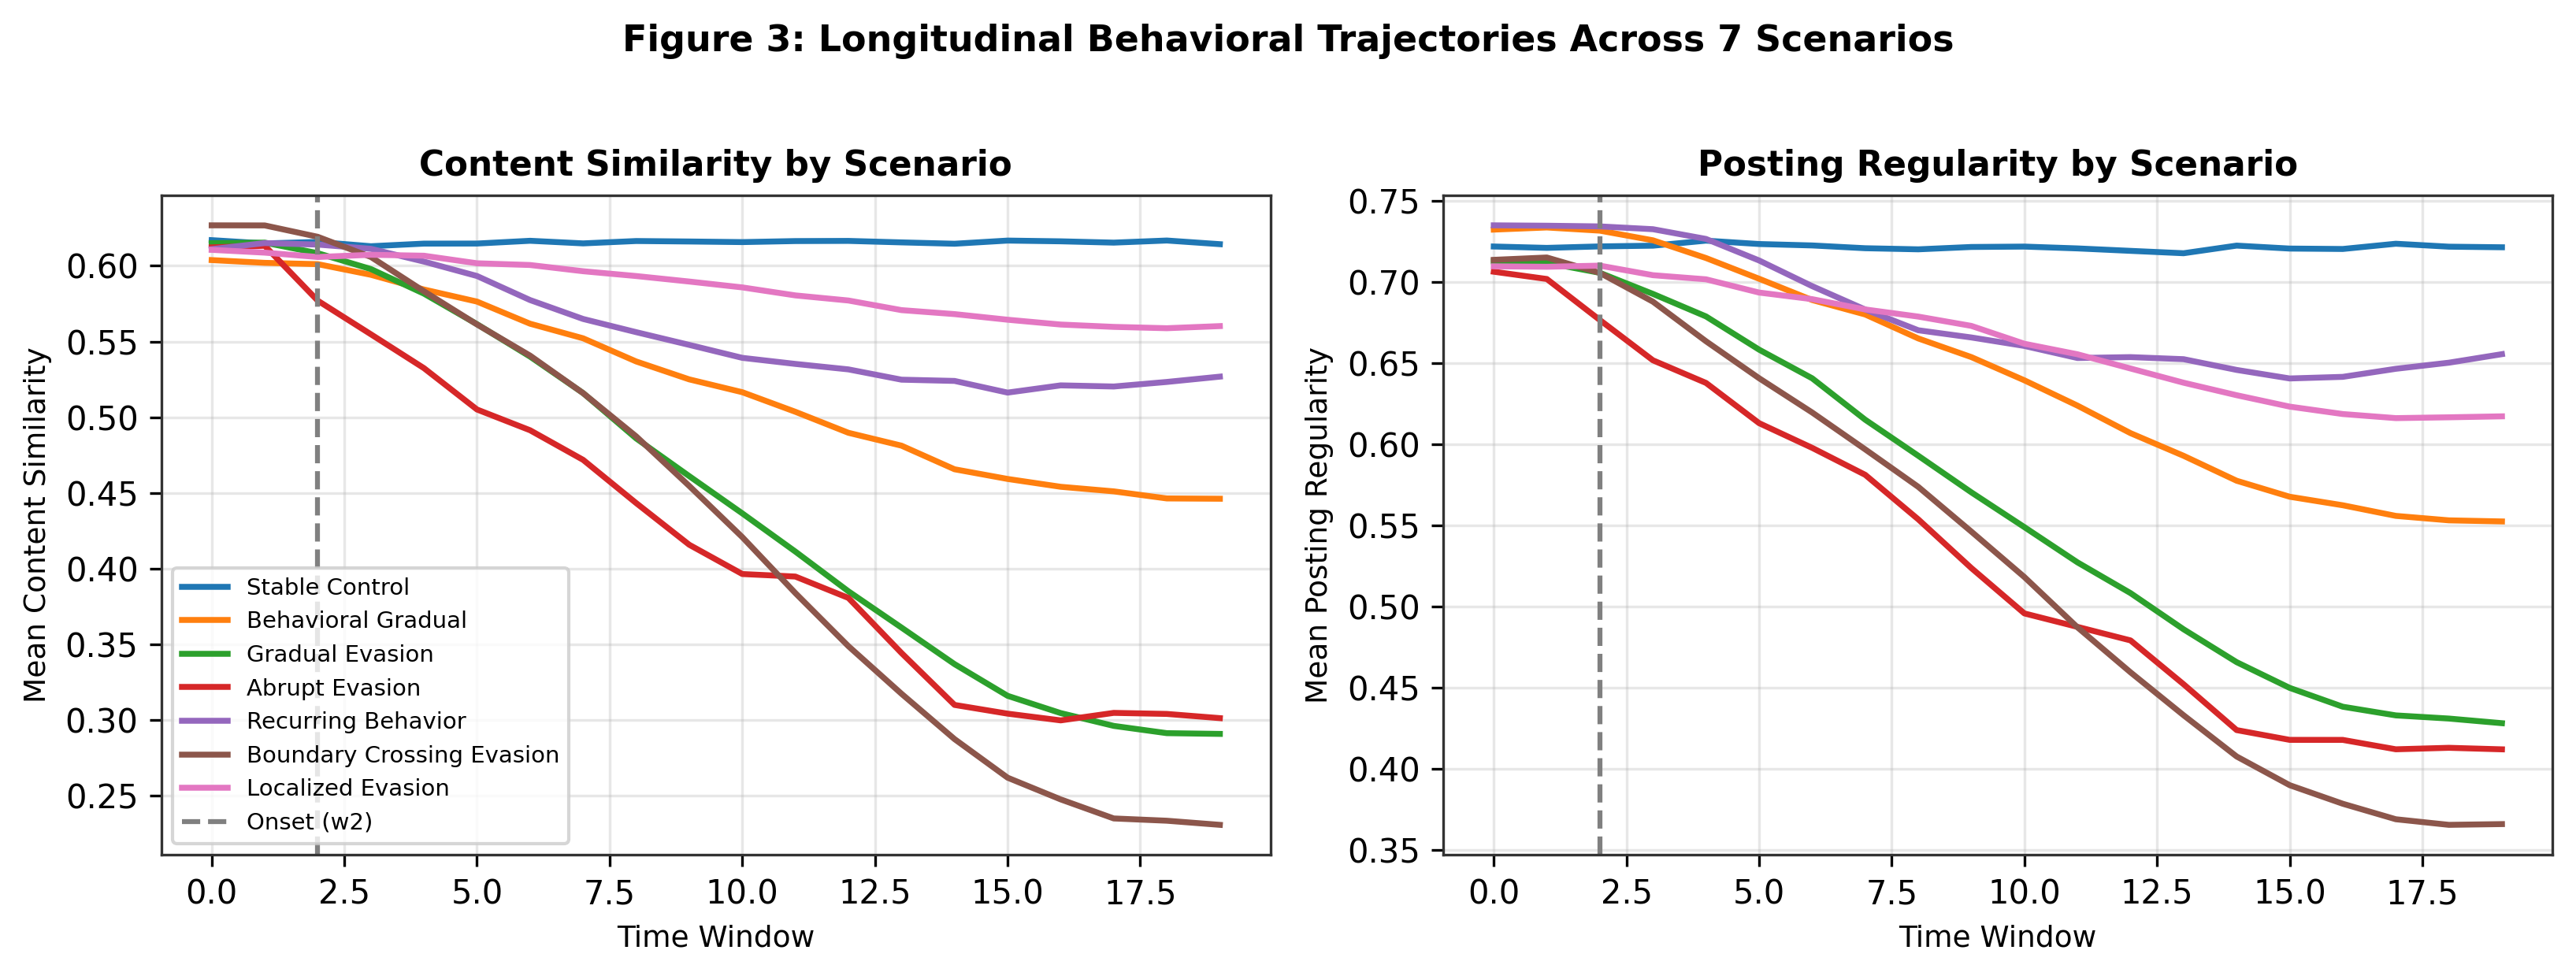
\includegraphics[width=\columnwidth]{paper_pictures/fig3_temporal_drift_profiles.png}
\caption{Longitudinal behavioral feature trajectories across 7 drift scenarios over 20 temporal windows, illustrating targeted evasion patterns.}
\label{fig:scenarios}
\end{figure}

Bot accounts are assigned across seven scenarios with proportions summing to 1.00:
\begin{enumerate}
    \item \textbf{stable\_control (13\%)}: Stationary baseline with zero drift across all 20 windows.
    \item \textbf{behavioral\_gradual (17\%)}: Organic drift in posting tempos and linguistic habits.
    \item \textbf{gradual\_evasion (26\%)}: Continuous migration toward human feature centroids.
    \item \textbf{abrupt\_evasion (10\%)}: Step-function transition at onset window toward human activity.
    \item \textbf{localized\_evasion (8\%)}: Targeted evasion restricted to specific feature subsets.
    \item \textbf{recurring\_behavior (6\%)}: Cyclic oscillation between automated and human activity modes.
    \item \textbf{boundary\_crossing\_evasion (20\%)}: Adversarial shift specifically configured to breach the initial static decision boundary.
\end{enumerate}

\section{Benchmark Validation and Baseline Evaluation}

\begin{figure}[!t]
\centering
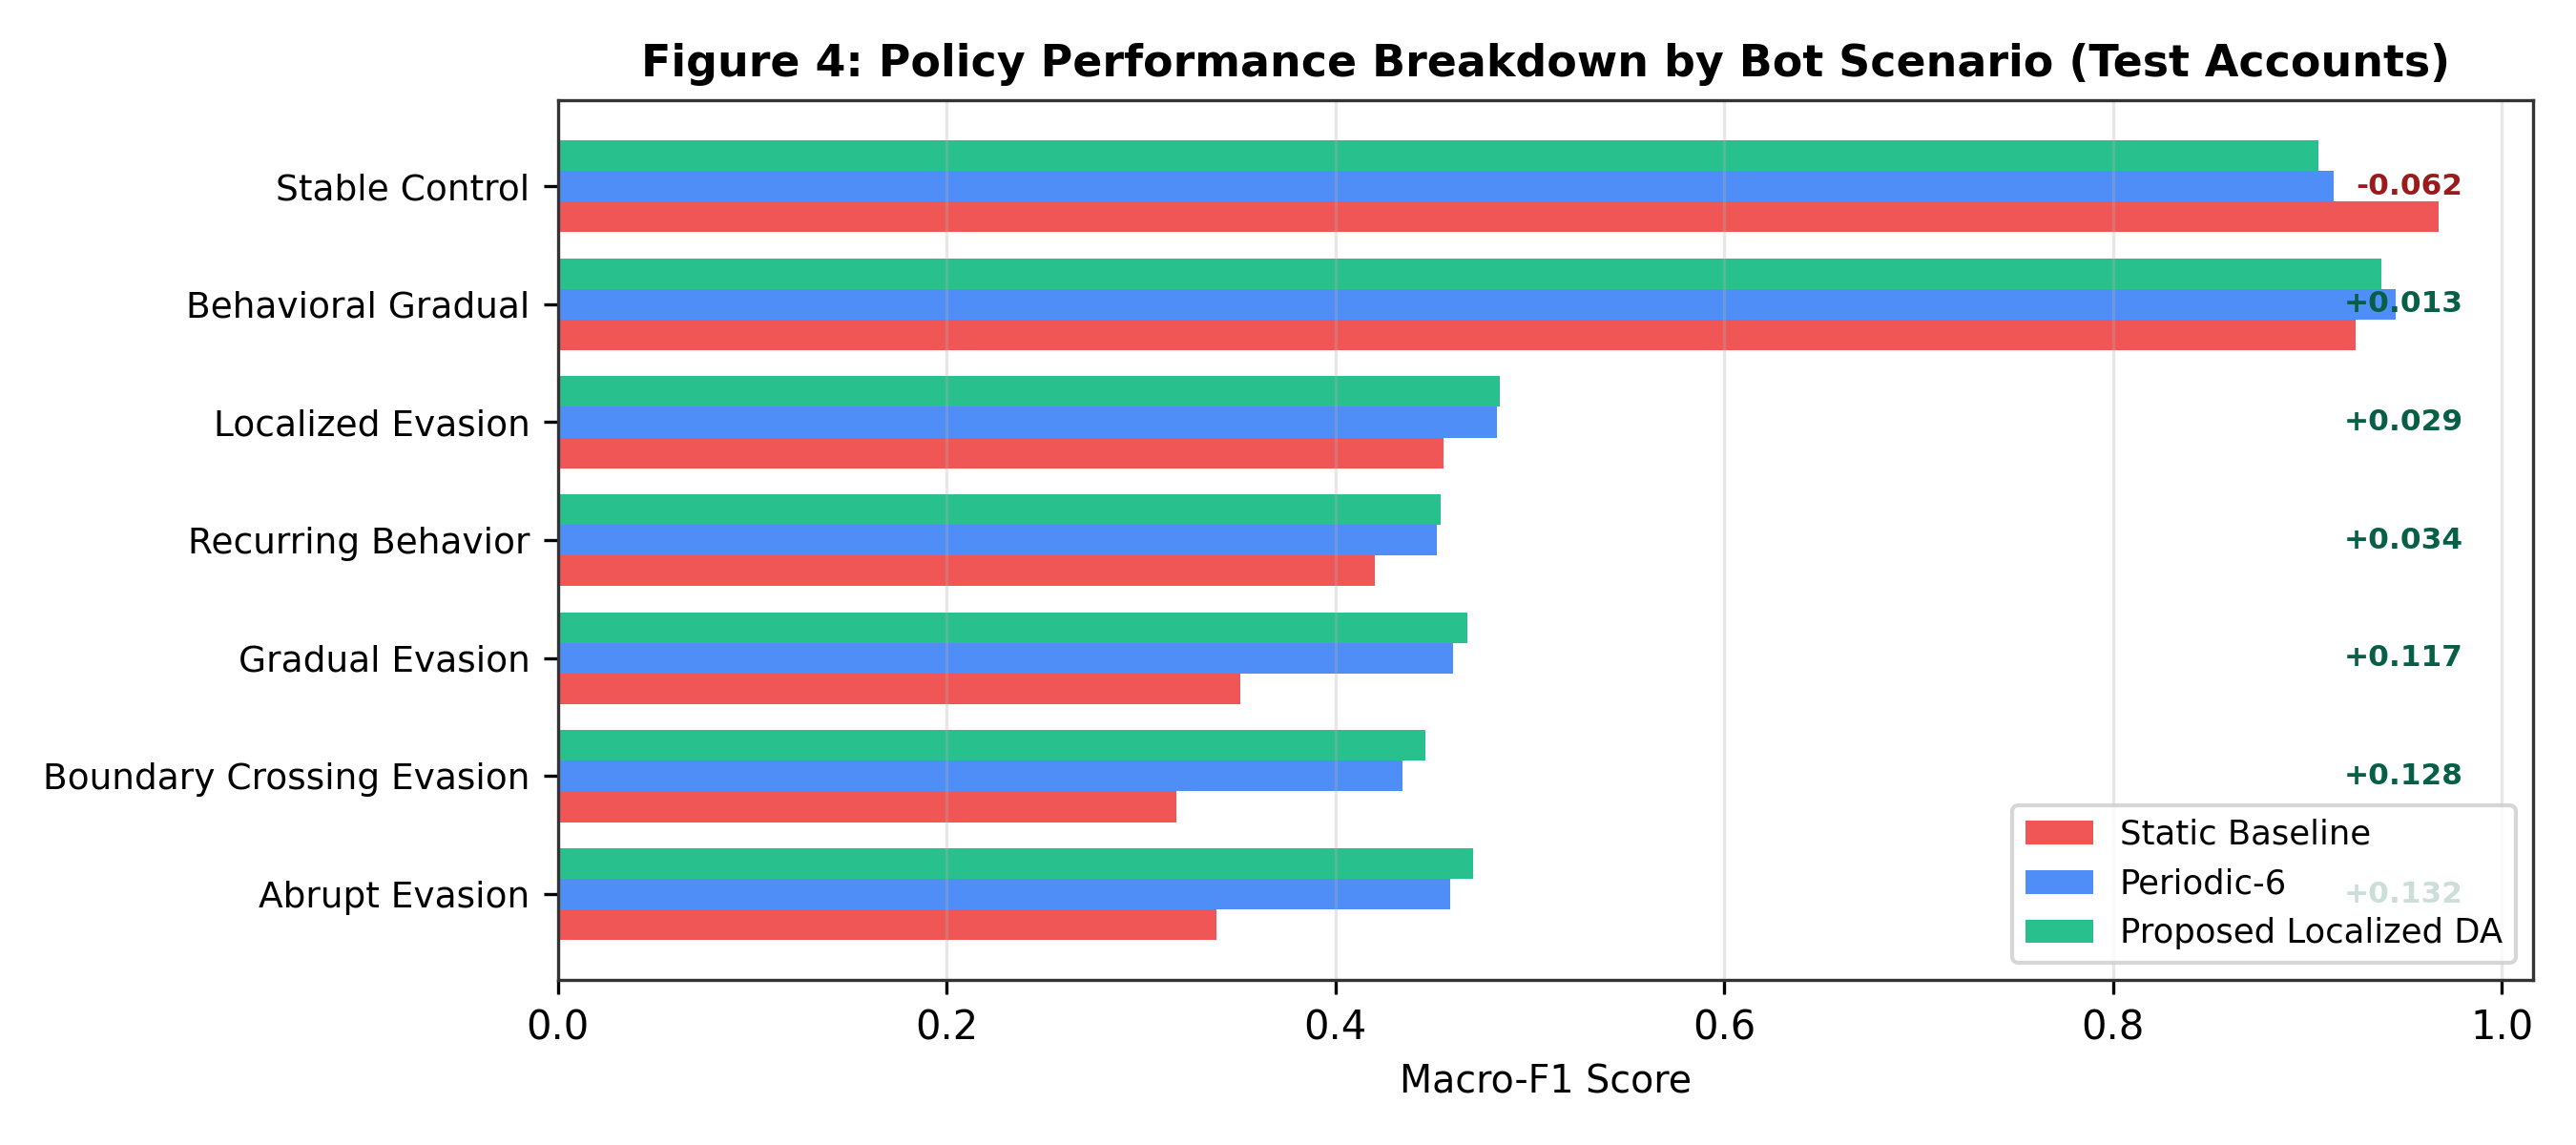
\includegraphics[width=\columnwidth]{paper_pictures/fig4_scenario_degradation_heatmap.png}
\caption{Policy performance breakdown across all 7 bot scenarios on held-out test accounts, demonstrating severe static degradation and adaptive recovery.}
\label{fig:heatmap}
\end{figure}

We benchmarked baseline classifiers using an account-disjoint 3-way split (1,800 train / 600 validation / 600 test accounts) across 5 independent seeds (2025--2029):
\begin{itemize}
    \item \textbf{Pre-Drift Performance}: The static baseline achieves Macro-F1 = 0.9770 $\pm$ 0.0008, confirming high baseline separability.
    \item \textbf{Post-Drift Degradation}: Static performance drops to Macro-F1 = 0.8059 $\pm$ 0.0015 (worst window F1 = 0.6583), driven by a collapse in bot recall to 67.26\% (and 35.40\% at window 18).
    \item \textbf{Scenario Degradation (Fig.~\ref{fig:heatmap})}: Evasion scenarios experience severe drops in static F1 (down to 0.318--0.351), while the stationary control group remains at F1 = 0.9677.
    \item \textbf{Adaptive Recovery}: Localized drift-aware adaptation restores temporal Macro-F1 to 0.9167 $\pm$ 0.0009 and bot recall to 89.31\%.
\end{itemize}

\section{Discussion}
\subsection{Synthetic Ground Truth vs. Platform Heuristics}
Controlled synthetic benchmarks provide an indispensable experimental testbed for concept drift research. In observational platform streams, true account labels are unobservable over time without account suspension telemetry (which introduces survivor bias). BotDriftBench provides known onset coordinates and affected feature subsets, enabling exact evaluation of detector sensitivity, latency, and attribution accuracy.

\subsection{Preserving Empirical Correlation Structures}
A recurring flaw in synthetic tabular generators is the independent sampling of individual feature dimensions, which creates impossible ``chimera'' accounts. By sampling complete empirical training rows to build human reference manifolds, BotDriftBench preserves realistic covariance relationships between account age, follower counts, and posting volume.

\subsection{Organic Growth vs. Artificial Interpolation}
Separating structural profile growth from behavioral evasion mirrors real-world constraints: while bot operators can easily modify posting tempos, text diversity, and URL sharing rates overnight, they cannot rewrite account registration age or fabricate organic historical growth.

\section{Limitations}
\begin{enumerate}
    \item \textbf{Approximated Higher-Order Interactions}: While marginals and empirical row pairs are preserved, multi-account coordinated network topology is simplified.
    \item \textbf{Platform Context}: Features reflect Twitter/X style microblogging and may require re-calibration for other platforms.
\end{enumerate}

\section{Conclusion and Data Availability}
BotDriftBench v0.8 provides the first calibrated longitudinal benchmark with controlled drift ground truth, organic growth dynamics, and strict account-disjoint evaluation protocols. The dataset, configuration manifest, and baseline generation code are released under CC BY 4.0 at: \url{https://github.com/esh22nika/bot_detection}.

\bibliographystyle{IEEEtran}
\bibliography{references}

\end{document}
